\documentclass[10pt,twoside,slovak,a4paper]{article}

\usepackage[slovak]{babel}
\usepackage[IL2]{fontenc}
\usepackage[utf8]{inputenc}
\usepackage{graphicx}
\usepackage{url}
\usepackage{hyperref}
\usepackage{cite}

\pagestyle{headings}

\title{Path of Exile a role-playing games} 

\author{Mário Babiar\\[2pt]
	{\small Slovenská technická univerzita v Bratislave}\\
	{\small Fakulta informatiky a informačných technológií}\\
	{\small \texttt{xbabiar@stuba.sk}}
	}

\date{\small 11. októbra 2022}

\begin{document}
\maketitle

\begin{abstract}
Článok sa zameriava na Path of Exile (PoE) od štúdia Grinding Gear Games (GGG) a action role-playing hry (ARPG). 1) Vysvetľuje Path of Exile, jej históriu, charakteristické herné prvky a monetizáciu. 2) Porovnáva Path of Exile s inými hrami zo žánru ARPG alebo RPG ako Diablo II a Diablo III. 3) Hodnotí v čom Path of Exile vyniká a prečo je jedna z najlepších hier vo svojom žánri, ale aj v čom zaostáva.
\centering
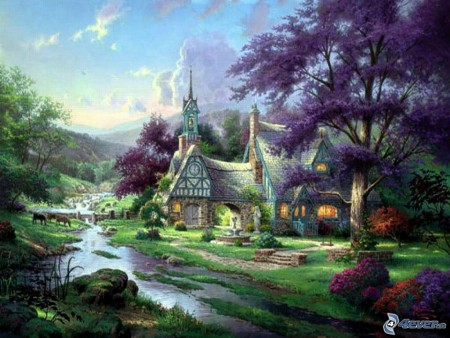
\includegraphics[scale=0.5,]{obrazok.jpg}
\end{abstract}
\section{Obrázok}
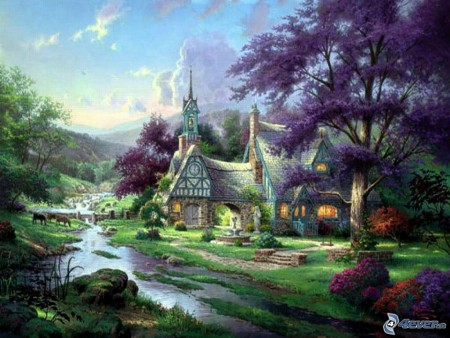
\includegraphics[scale=0.5]{obrazok.jpg}
\end{document}
